\documentclass[a4j,12pt]{jarticle}

\usepackage[margin=0.5in]{geometry}
\usepackage{ascmac}
\usepackage{amsmath}
\usepackage{amssymb}
\usepackage{amsthm}
\usepackage{fancybox}
\usepackage{float}
\usepackage{subcaption}
\usepackage{mathrsfs}
\usepackage[dvips,final]{graphicx}
\usepackage{tabularx}
\usepackage{enumerate}
\usepackage{tikz}
\usetikzlibrary{positioning}

\numberwithin{equation}{section}
\newtheorem{example}{例}[section]

\newcommand{\N}{\mathbb N}
\newcommand{\R}{\mathbb R}
\newcommand{\C}{\mathbb C}
\newcommand{\bra}[1]{\langle{#1}|}
\newcommand{\ket}[1]{|{#1}\rangle}
\newcommand{\Expect}[3]{\langle {#1}|{#2}|{#3} \rangle}
\newcommand{\dev}[2]{\langle (\Delta {#1})^2 \rangle _{{#2}}}
\newcommand{\sgm}[1]{\sigma_{#1}}
\newcommand{\sgmOp}[1]{\hat{\sigma}_{#1}}
\newcommand{\hfangle}[1]{{\frac{#1}{2}}}
\newcommand{\clmnV}[2]
		{\left(
			\begin{matrix}
			 {#1}\\
			 {#2}\\
		 	\end{matrix}
		\right)
		}
\newcommand{\clmnVsan}[3]
		{\left(
			\begin{matrix}
			 {#1}\\
			 {#2}\\
			 {#3}\\
		 	\end{matrix}
		\right)
		}
\newcommand{\mtrx}[4]
	{\left(
		\begin{matrix}
		 {#1} & {#2} \\
		 {#3} & {#4} \\
		\end{matrix}
	\right)
	}
\newcommand{\inn}[2]{\langle{#1}|{#2}\rangle}
\newcommand{\itbf}[1]{\textit{\textbf{#1}}}

\newtheorem{dfn}{定義}[section]
\newtheorem{thm}{定理}[section]
\newtheorem{prop}[thm]{命題}
\newtheorem{lemma}[thm]{補題}
\renewcommand{\proofname}{\textbf{証明}}

\begin{document}
\title{Pointless Topology 勉強ノート}
\date{2024年6月13日〜}
\author{中村仁宣}
\maketitle

\section{Preliminary}
\subsection{Topology トポロジー}
Let $\mathcal{P}(X)$ denote the power set of $X$.
\begin{dfn}[Topology トポロジー]
  A \itbf{topological space} is an ordered pair $(X, \tau), \; \tau \subseteq \mathcal{P}(X)$ which satisfies the following properties
  \begin{enumerate}
  \item $\varnothing \in \tau$ and $X \in \tau$.
  \item if $U,V \in \tau$, then $U \cap V \in \tau$.
  \item if $\forall I, U_i \in \tau \text{ forall } i \in I$, then $\bigcup_{i\in I}U_i$.
  \end{enumerate}
  $\tau$ is called the \itbf{topology} of $X$.
  The members of the topology $U\in\tau$ is said to be \itbf{open} and $V \subseteq X$ is said to be \itbf{closed} if $\exists U$ open such that $V = U^c$.
\end{dfn}
\begin{dfn}
  If $X$ is a topological space and $x \in X$, a neighbourhood (abbreviated ``nhood``) od $x$ is a set $U$ which contains an open set $V$ containing $x$.
  Thus, $U$ is a nhood of $x$ iff $x \in U^{\circ}$.
  The collection $\mathscr{U}_x$ of all nhoods of $x$ is the nhood system of $x$.
\end{dfn}
\begin{dfn}[Separation Axioms 分離公理]
  A space $(X,\tau)$ is called $T_i$ ,if respectively satisfies the following conditions,
  \begin{enumerate}
  \item $T_0$: $\forall x,y \in X$ $\exists$ an open set $U \in \tau$ such that $U$ contains one of $x,y$ and not the other.
  \item $T_1$: $\forall x,y \in X$ $\exists$ a nhood of each not containing the other.
  \end{enumerate}
\end{dfn}
\begin{example}[$T_0$-space]
  $X=\{a,b\}, \tau=\{\varnothing, \{a\}, X\}$
\end{example}
\subsection{Posets, Lattices 半順序集合、束}
\begin{dfn}[Posets]
  A \itbf{partial order (半順序)} on a set $X$ is a binary relation $R \subseteq X \times X$ satisfying,
  \begin{enumerate}
  \item $\forall a, aRa$ (reflexivity, 反射律),
  \item $\forall a,b,c,\; aRb \; \& \; bRc \Rightarrow aRc$ (transitivity, 推移律),
  \item $\forall a,b,\; aRb \; \& \; bRa \Rightarrow a=b$ (antisymmetry, 反対称律).
  \end{enumerate}
  if moreover
  \begin{enumerate}
    \setcounter{enumi}{3}
  \item $\forall a,b$ either $aRb$ or $bRa$ holds,
  \end{enumerate}
  it is said to be a \itbf{linear} or \itbf{total} order.\\
  A \itbf{poset} or \itbf{partially ordered set}, $(X, \le)$ is a set with a partial order.
  If the order of a poset is linear (or total), it is called a \itbf{linearly ordered set}, \itbf{totally ordered set} or \itbf{chain}.
  A relation that satisfies only (1) and (2) is called \itbf{preorder}.
\end{dfn}
\begin{dfn}[Suprema, infima]
  A \itbf{supremum} $s$ of a subset $M \subseteq (X, \le)$ the least upper bound of $M$, that is
  \begin{enumerate}
  \item $\forall m \in M, m \le s,$
  \item $\forall m \in M, m \le x \Rightarrow s \le x$.
  \end{enumerate}
  Similarly, a \itbf{infimum} of a subset $M \subseteq (X, \le)$ the greatest lower bound of $M$.\\
  We also call a supremum a \itbf{join} and an infimum \itbf{meet} and notate $\sup M, \inf M$ or $\bigvee M, \bigwedge M$ respectively.\\
  For finite cases, we wirte $a \vee b := \sup\{a,b\}$ or $a_1 \vee \dots \vee a_n := \sup\{a_1\dots a_n\}$ and $a \wedge b := \inf\{a,b\}$ or $a_1 \wedge \dots \wedge a_n := \inf\{a_1\dots a_n\}$.
\end{dfn}
Since each $x\in X$ is both a lower and an upper bound of the empty set $\varnothing$,
\begin{equation}
  \sup\varnothing \text{ is the least element of } X
\end{equation}
and
\begin{equation}
  \inf\varnothing \text{ is the greatest element of } X
\end{equation}
We use the symbols $0$ or $\bot$ for the former and $1$ or $\top$ for the latter.\\
\begin{dfn}[Semilattices, Lattice]
  A \itbf{meet-semilattice} is a poset $X$ such that $\forall a,b \in X$ there exists an infimum $a \wedge b$.\\
  A \itbf{join-semilattice} is a poset $X$ such that $\forall a,b \in X$ there exists an supremum $a \vee b$.\\
  A \itbf{lattice} is a poset $X$ such that $\forall a,b \in X$ both an infimum $a \wedge b$ and a supremum $a \vee b$ exist.\\
  A \itbf{bounded lattice} is a poset in which all finite subsets have infima and suprema (i.e. a lattice with bottom and top).\\
  A poset is a \itbf{complete lattice} if every subset has a supremum and an infimum.
\end{dfn}
In a bounded semilattice, $\wedge$ or $\vee$ is a binary operation and satisfies the following properties,
\begin{align}
  & a \wedge a = a && a \vee a = a\\
  & a \wedge b = b \wedge a &&  a \vee b = b \vee a \\
  & (a \wedge b) \wedge c = a \wedge (b \wedge c)  && (a \vee b) \vee c = a \vee (b \vee c) \\
  & a \wedge 1 = a && a \vee 0 = a.
\end{align}
In other words, bounded semilattices are commutative monoids (semigroup with unit/identity element) in which every element is idempotent.\\
\begin{thm} \label{thm:comm-monoid-is-lattice}
  Let $(A, \vee, 0)$ be a commutative monoid in which every element is idempotent.
  Then there exists a unique partial order on $A$ such that $a \wedge b$ is the join of $a$ and $b$, and $0$ is the least element.
\end{thm}
\begin{proof}
  If such a partial order exists,
  \begin{equation}
    a \le b \Leftrightarrow a \vee b = b.
  \end{equation}
  would be the correspondence. Now, let us verify this connection.\\
  \itbf{Reflexivity}\\
  \begin{equation}
   a \wedge a = a \Rightarrow a \le a.
  \end{equation}
  \itbf{Antisymmetry}\\
  If $a \le b$ and $b \le a$, then $b = a \wedge b = b \wedge a = a$ by commutativity.\\
  \itbf{Transitivity}\\
  If $a \le b$ and $b \le c$, then
  \begin{align*}
    a \wedge c &= a \wedge (b \wedge c) & (\because b \le c)\\
               &= (a \wedge b) \wedge c & (\text{associativity})\\
               &= b \wedge c & (\because a \le b)\\
               &= c & (\because b \le c)
  \end{align*}
  Hence, $a \le c$.\\
  \itbf{Join-uniqueness}\\
  Since $a \wedge (a \wedge b) = (a \wedge a) \wedge b = a \wedge b$, $a \le a \wedge b$.
  Similarly, $b \le a \wedge b$, so $a \wedge b$ is an upper-bound for $\{a,b\}$. For the leastness, suppose $a \le c$ and $b \le c$, then 
  \begin{align*}
    (a \wedge b) \wedge c &= a \wedge (b \wedge c)\\
                          &= a \wedge c\\
                          &= c.
  \end{align*}
  Hence, $a \wedge b \le c$.
\end{proof}
A lattice can also be defined purely algebraically in those terms,
\begin{dfn}
  A \itbf{lattice} $(L, \vee, \wedge)$ is an algebra (a set with two binary operations) that satisfy
  \begin{align*}
    \label{eq:lattice-def}
    & (L1) &  & a \wedge a = a && a \vee a = a                       &  & \text{(idempotency)}   \\
    & (L2) &  & a \wedge b = b \wedge a && a \vee b = b\vee a        &  & \text{(commutativity)} \\
    & (L3) &  & (a \wedge b) \wedge c = a \wedge (b \wedge c)       &  & (a \vee b) \vee c = a \vee (b\vee c)                 &  & \text{(associativity)} \\
    & (L4) &  & a \vee (a \wedge b) = a && a \wedge (a \vee  b) =  a &  & \text{(absorption identities)}
  \end{align*}
\end{dfn}
($L4$) is necessary for the two operations $\wedge, \vee$ to be consistent with the corresponding order $\le$.
In fact, $a\wedge b = b$ implies $a \vee b = a \vee ( a \wedge b) = a$ by ($L4$).\\
For homomorphisms (structure-preserving maps) of (semi)lattices and posets, we need to be a little bit careful since the order-preserving homomorphisms of posets does not always preserve the joins (or meets) as shown in the following example.(\cite{Stone} section 1.3 Exercise)
%---Example---%
\begin{example}
  Consider the posets $X=\{a \le c, b \le c\}$ and $Y=\{e \le g, f \le g, g \le h\}$, and a homomorphism $\phi : X \rightarrow Y$ which maps each element as in the diagram below:
\begin{figure}[H]
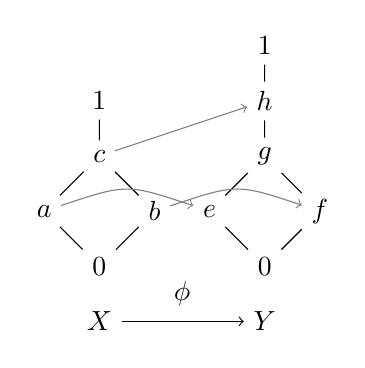
\begin{tikzpicture}[scale=.7]
  \node (one) at (0,2) {$1$};
  \node (a) at (-1,0) {$a$};
  \node (b) at (1,0) {$b$};
  \node (c) at (0,1) {$c$};
  \node (zero) at (0,-1) {$0$};
  \node (X) at (0,-2) {$X$};
  \node (one') at (3,3) {$1$};
  \node (e) at (2,0) {$e$};
  \node (f) at (4,0) {$f$};
  \node (g) at (3,1) {$g$};
  \node (h) at (3,2) {$h$};
  \node (zero') at (3,-1) {$0$};
  \node (Y) at (3,-2) {$Y$};
  \node (phi) at (1.5,-1.5) {$\phi$};
  \draw (zero) -- (a) -- (c);
  \draw (zero) -- (b) --  (c) -- (one);
  \draw (zero') -- (e) -- (g);
  \draw (zero') -- (f) --  (g) -- (h) -- (one');
  \draw[gray,->] (a) .. controls (0.5,0.5)..  (e);
  \draw[gray,->] (b) .. controls (2.5,0.5)..  (f);
  \draw[gray,->] (c) .. controls (1.5,1.5)..  (h);
  \draw[->] (X) -- (Y);
\end{tikzpicture}
\end{figure}  
Indeed, we have $a, b\le c$ and $\phi(a), \phi(b) \le \phi(c)$, which means the order is preserved, but $\phi(a \vee b) \ne \phi(a) \vee \phi(b)$.
\end{example}
(\cite{Stone} Sec.1.5) In most of the lattices we'll consider, the operations $\wedge$ and $\vee$ will satisfy an additional identity, namely the distributive law
\begin{equation}
  \label{eq:distributivity}
  \text{(i) } a \wedge (b \vee c) = (a \wedge b) \vee (a \wedge c)
\end{equation}
for all $a,b,c$.
\begin{lemma}
  If the distributive law (i) holds in a lattice, then so does its dual, i.e. the identity
  \begin{equation}
    \label{eq:ditributivity2}
    \text{(ii) } a \vee (b \wedge c) = (a \vee b) \wedge (a \vee c)
  \end{equation}
\end{lemma}
\begin{proof}
  \begin{align*}
    (a \vee b) \wedge (a \vee c) &= ((a \vee b) \wedge a) \vee ((a \vee b) \wedge c) &\text{by (i)}\\
                                 &= a \vee ((a \wedge c) \vee (b \wedge c)) &\text{by absorption law}\\
                                 &= a \vee (b \wedge c) &\text{by absorption law}
  \end{align*}
\end{proof}
Note also that in the presence of (i), we can deduce either of the two absorptive law from the other,
\begin{equation}
  a \wedge (a \vee b) = (a \wedge a) \vee (a \wedge b) = a \vee (a \wedge b)
\end{equation}
\begin{prop}
  Let $a,b,c$ be three elements of a distributive lattice $A$. Then there exists at most one $x \in A$ satisfying $x \wedge a = b$ and $x \vee a = c$.
\end{prop}
\begin{proof}
  Suppose both $x$ and $y$ satisfy the conditions. Then,
  \begin{align*}
    x &= x \wedge (x \vee a) = x \wedge c = x \wedge (y \vee a) \\
      &= (x \wedge y) \vee (x \wedge a)\\
      &= (x \wedge y) \vee b = x \wedge y
  \end{align*}
  since $b = x \wedge a = y \wedge a$ is a lower bound for $\{x,y\}$. Similarly, we have $y = x \wedge y$; so $x=y$.
\end{proof}
In any lattice, an element $x$ satisfying $x\wedge a = 0$ and $x \vee a = 1$ is called a \itbf{complement} of $a$.
The Porposition above tells us that in a distributive lattice, complements are unique when they exist.
A \itbf{Boolean algebra} is a distributive lattice $A$ equipped with an additional unary operation $\neg :A \rightarrow A$ such that $\neg a$ is a complement of $a$.
Since $\neg$ is uniquely determined by the other data in the definition, it follows that any lattice homomorphism $f:A\rightarrow B$ between Boolean algebras is actually a Boolean algebra homomorphism(i.e. commutes with $\neg$).
\begin{example}[Power set]
  For any set $X$, the power set $\mathcal{P}(X)$ of $X$ is a lattice, with $\le$ interpreted as inclusion, $\wedge$ and $\vee$ as union and intersection of subsets, and $0$ and $1$ as the empty set and the whole of $X$. Moreover $\mathcal{P}(X)$ is distributive. Since $\mathcal{P}(X)$ has complements for all its elements, it is a Boolean algebra.
\end{example}
\begin{example}[Total Order]
  Let $A$ be a totally ordered set with least and greatest elements $0$ and $1$. Then $A$ is a lattice, with $\wedge$ and $\vee$ interpreted as $\min$ and $\max$. It is distributive;
  \begin{equation}
    \min\{a, \max\{b,c\}\} = \max\{\min\{a,b\}, \min\{a,c\}\}
  \end{equation}
  But if $A$ has more than two elements, it is not a Boolean elgebra; for no element other than $0$ and $1$ can have a complement.
\end{example}
\begin{example}[Lattices of subgroups]
  Let $G$ be a group. The set subgroups of $G$, ordered by inclusion, is a lattice in which meet is again interpreted as intersection, but the join of two subgroups is the subgroup generated by their union.
  This lattice is not in general distributive; for example, if $G$ is the non-cyclic group of order 4, the lattice looks like
  \begin{figure}[H]
    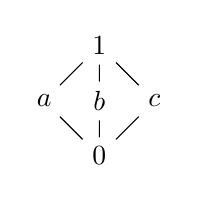
\begin{tikzpicture}[scale=.7]
      \node (one) at (0,1) {$1$};
      \node (a) at (-1,0) {$a$};
      \node (b) at (0,0) {$b$};
      \node (c) at (1,0) {$c$};
      \node (zero) at (0,-1) {$0$};
      \draw (zero) -- (a) -- (one) -- (b) -- (zero) -- (c) -- (one);
    \end{tikzpicture}
  \end{figure}
  where $a,b,c$ are the three subgroups of order 2, and each of $a,b,c$ has two distict complements.
\end{example}
\subsubsection{Boolean Rings and Boolean algebras}
\begin{prop}
  De Morgan's law
  \begin{align*}
    \neg (x \wedge y) = \neg x \vee \neg y
  \end{align*}
  holds.
\end{prop}
\begin{proof}
  We need to say that $\neg x \vee \neg y$ is the complement of $x \wedge y$,
  \begin{align*}
    & (\neg x \vee \neg y)\wedge (x \wedge y) \\
    &= ((\neg x \wedge x \wedge y) \vee (\neg y \wedge x \wedge y)) \\
    &= (0 \wedge y) \vee (0 \wedge x) \\
    &= 0
  \end{align*}
  \begin{align*}
    & (\neg x \vee \neg y)\vee (x \wedge y) \\
    &= (\neg x \vee \neg y \vee x) \wedge (\neg x \vee \neg y \vee y) \\
    &= (1 \vee y) \vee (1 \vee x) \\
    &= 1
  \end{align*}
\end{proof}
Next, we sketch the equivalence between Boolean algebras and Boolean rings. In any Boolean algebra $A$, we define the \itbf{symmetry difference} operation $+$ by
\begin{equation}
  a + b = (a\wedge \neg b) \vee (b \wedge \neg a).
\end{equation}
\begin{lemma}
  \label{lemma:B-alg-distributivity}
  The distributive law $a \wedge (b+c) = (a\wedge b) + (a \wedge c)$
\end{lemma}
\begin{proof}
  \begin{align*}
    (a \wedge b) + (a \wedge c) &= ((a \wedge b) \wedge \neg (a \wedge c)) \vee ((a \wedge c) \wedge \neg (a \wedge b)) \\
                                &= ((a \wedge b) \wedge (\neg a \vee \neg c)) \vee ((a \wedge c) \wedge (\neg a \vee \neg b)) \\
                                &= ((a \wedge b \wedge \neg a) \vee (a \wedge b \wedge \neg c)) \vee ((a \wedge c \wedge \neg a) \vee (a \wedge c \wedge \neg b)) \\
                                &= (0 \vee (a \wedge b \wedge \neg c)) \vee (0 \vee (a \wedge c \wedge \neg b)) \\
                                &= (a \wedge b \wedge \neg c) \vee (a \wedge c \wedge \neg b) \\
                                &= a \wedge ((b \wedge \neg c) \vee (c \wedge \neg b)) \\
                                &= a \wedge (b + c).
  \end{align*}
\end{proof}
\begin{lemma}
  The associative law
  \begin{equation}
    a+(b+c) = (a+b)+c
  \end{equation}
  holds.
\end{lemma}
\begin{proof}
  \begin{align*}
    a+(b+c) &= a+((b \wedge \neg c) \vee (c \wedge \neg b)) \\
            &= (a \wedge \neg ((b \wedge \neg c) \vee (c \wedge \neg b)) \vee (\neg a \wedge ((b \wedge \neg c) \vee (c \wedge \neg b))) \\
            &= (a \wedge ((\neg b \vee c) \wedge (\neg c \vee b)) \vee ((\neg a \wedge b \wedge \neg c) \vee (\neg a \wedge c \wedge \neg b)) \\
            &= (a \wedge ((\neg b \wedge \neg c) \vee (\neg b \wedge b) \vee (c \wedge \neg c) \vee (c \wedge b)) \vee ((\neg a \wedge b \wedge \neg c) \vee (\neg a \wedge c \wedge \neg b)) \\
            &= (a \wedge ((\neg b \wedge \neg c) \vee 0 \vee 0 \vee (c \wedge b)) \vee ((\neg a \wedge b \wedge \neg c) \vee (\neg a \wedge \neg b \wedge c)) \\
            &= (a \wedge \neg b \wedge \neg c) \vee (a \wedge c \wedge b) \vee (\neg a \wedge b \wedge \neg c) \vee (\neg a \wedge \neg b \wedge c) \\
            &= (((a \wedge \neg b) \vee (\neg a \wedge b )) \wedge \neg c) \vee (((a \wedge b) \vee  (\neg a \wedge \neg b)) \wedge c) \\
            &= ((a+b) \wedge \neg c) \vee (\neg ((a \wedge \neg b) \vee  (\neg a \wedge b)) \wedge c) \\
            &= ((a+b) \wedge \neg c) \vee (\neg (a+b) \wedge c) \\
            &= (a+b) + c.
  \end{align*}
\end{proof}
Now for any $a$, we have
\begin{equation}
  a+a=(a \wedge \neg a) \vee (a \wedge \neg a) = 0 \wedge 0=0
\end{equation}
\begin{equation}
  a + 0 = (a \wedge 1) \vee (0 \wedge \neg a) = a \vee 0 = a.
\end{equation}
So $(A, +, 0)$ is a commutative group, and $(A, +, \wedge, 0, 1)$ is a commutative ring with $1$.
\begin{dfn}
  A Boolean ring $A$ is a ring with $1$ in which every element satisfies $a^2 = a$.
\end{dfn}
\begin{lemma}
  Let $A$ be a Boolean ring, then
  \begin{enumerate}
  \item $A$ is commutative.
  \item Every $a \in A$ satisfies $a+a=0$.
  \end{enumerate}
\end{lemma}
\begin{proof}
  \begin{align*}
    a + b &= (a+b)^2 \\
          &= a^a + ab + ba + b^2 \\
          &= a + ab + ba + b.
  \end{align*}
  So $ab + ba = 0$. Putting $a=b$, we get $a+a=0$; hence $ab=-ba=ba$.
\end{proof}
So the multiplicative structure $(A, \cdot,1)$ is a semilattice, with partial order defined by $a \le b$ iff $ab=a$ (c.f. 定理 \ref{thm:comm-monoid-is-lattice}).
Note that $0$ is the least element of $A$ for this order.\\
Now consider $a+b+ab$. We have
\begin{equation}
  a(a+b+ab)=a+ab+ab=a
\end{equation}
and
\begin{equation}
  b(a+b+ab)=ba+b+ab=b
\end{equation}
so $a+b+ab$ is an upper bound for $\{a,b\}$. But if $c$ is an upper bound for $\{a,b\}$, then
\begin{equation}
  (a+b+ab)c=ac+bc+abc=a+b+ab,
\end{equation}
so $a+b+ab$ is the least upper bound. Dnote $a+b+ab$ by $a\vee b$, we thus havea lattice structure $(A, \vee, \cdot, 0, 1)$.
Moreover, by an argument like that of Lemma \ref{lemma:B-alg-distributivity}, we may verify that $\cdot$ is distributive over $\vee$;
and it is also easy to verify that $1+a$ is a complement for $a$. So $A$ is a Boolean algebra.
\begin{align*}
  ab \vee ac &= (ab+ac+abac) \\
               &= ab + ac + abc \\
               &= a(b \vee c) &\text{\qed}
\end{align*}
\begin{align*}
  &a(a+1) = a+a=0 & a \vee (1+a) = a + (1+a) + a(1+a) = 1. &\text{\qed}
\end{align*}
What is the symmetric difference operation in this Boolean algebra?
\begin{align*}
  (a \wedge \neg b) \vee (b \wedge \neg a) &= (a (1+b)) \vee (b (1+a)) \\
                                           &= (a+ab) \vee (b+ab) \\
                                           &= (a+ab) + (b+ab) + (a+ab)(b+ab) \\
                                           &= a + b + ab + ab + ab + ab \\
                                           &= a + b.
\end{align*}
Thus if we start from a Boolean ring and turn it into a Boolean algebra by the definitions
\begin{align*}
  a \vee b &:= a + b +ab \\
  \neg a &:= 1 + a \\
  a \overline{+} b &:= a + b
\end{align*}
then back into a Boolean ring by defining the addition $+$ as the symmetric difference, we recover the original ring.
Similarly if start from a Boolean algebra and go round the other way.
Moreover, it is clear from the nature of the constructions that any Boolean algebra homomorphism is also a Boolean ring homomorphism, conversely; so we have proved
\begin{thm}
  The category of Boolean algebras is isomorphic to the category of Boolean rings.
\end{thm}
\subsection{Heyting Algebras ヘイティング代数}
Let $a$ and $b$ be elements of a Boolean algebra, and consider the element $\neg a \vee b$.
We have
\begin{align*}
  c \le \neg a \vee b \Rightarrow c \wedge a &\le a \wedge (\neg a \vee b) \\
                                             &=(a \wedge \neg a) \vee (a \wedge b) \\
                                             &=0 \vee (a \wedge b) = a \wedge b \\
                                             &\le b;
\end{align*}
and conversely
\begin{align*}
  c \wedge a \le b \Rightarrow \neg a \vee b &\ge \neg a \vee (a \wedge c) \\
                                             &=(\neg a \vee a) \wedge (\neg a \vee c) \\
                                             &=1 \wedge (\neg a \vee c) = \neg a \vee c \\
                                             &\ge c.
\end{align*}
Thus $\neg a \vee b$ is the unique largest element $c$ satisfying $c \wedge a \le b$. A lattice $A$ is said to be a \itbf{Heyting algebra} if, for each pair of elements $(a,b)$, there exists an element $(a \rightarrow b)$ such that $c\le(a\rightarrow b)$ iff $c \wedge a \le b$.
\begin{lemma}
  Let $A$ be a lattice, $\rightarrow$ a binary operation on $A$. Then $\rightarrow$ makes $A$ into a Heyting algebra iff the equations
  \begin{align*}
    &\text{(i) } a \rightarrow a =1 \\
    &\text{(ii) } a \wedge (a \rightarrow b) = a \wedge b \\
    &\text{(iii) } b \wedge (a \rightarrow b) = b \\
    &\text{(iv) } a \rightarrow (b \wedge c) = (a \rightarrow b) \wedge (a \rightarrow c)
  \end{align*}
  hold for all $a,b,c$ in $A$.
\end{lemma}
\begin{proof}
  Suppose that $A$ is a Heyting algebra. Then, $(a \rightarrow a)$ is the largest element $c$ such that $c \wedge a \le a$ holds, that is $1$. So (i) is true.\\
  For (ii), $a \wedge c \le b$ implies $a \wedge (a \wedge c) = a \wedge c \le a \wedge b$. Hence, $a \wedge (a \rightarrow b) \le a \wedge b$. Also, since $(a \wedge b) \wedge a \le b$, we have $a \wedge b \le a \rightarrow b \; \Rightarrow a \wedge b \le a \wedge (a \rightarrow b)$. So (ii) is true.\\
  For (iii), $a \wedge b \le b$ implies $b \le (a \rightarrow b)$, so $b \le b \wedge (a \rightarrow b) \le b$.\\
  For (iv), $a \wedge f \le (b \wedge c) \le b, c$ so $a \rightarrow (b \wedge c) \le (a \rightarrow b) \wedge (a \rightarrow c)$.\\
  Then $a \wedge (a \rightarrow b) \wedge (a \rightarrow c) = a \wedge (a \rightarrow b) \wedge a \wedge (a \rightarrow c) \le b \wedge c$, so it's true.\\
  For the converse, suppose the equations hold. Then if $c \le (a \rightarrow b)$, we have
  \begin{align*}
    a \wedge c \le a \wedge (a \rightarrow b) \le a \wedge b \le b
  \end{align*}
  conversely, if $c \wedge a \le b$ then
  \begin{align*}
    c &= c \wedge (a \rightarrow c) & \text{by (iii)} \\
      &\le(a \rightarrow a) \wedge (a \rightarrow c) & \text{by (i)} \\
      &=a \rightarrow (a \wedge c) & \text{by (iv)} \\
      &\le a \rightarrow b
  \end{align*}
  since $a \rightarrow (-)$ is order-preserving;\\
  $\because$ if $b \le c$ then $b = b \wedge c$
  \begin{align*}
    a \rightarrow b &= a \rightarrow (b \wedge c) \\
                    &= (a \rightarrow b) \wedge (a \rightarrow c)
  \end{align*}
  Hence, $a \rightarrow b \le a \rightarrow c$.
\end{proof}
(\cite{Stone} Sec. 1.11) In a Boolean algebra $A$, we can recover the unary operation $\neg$ from the binary operation $\rightarrow$, since $\neg a = (a \rightarrow 0)$.\\
$\because$ In a Boolean algebra, $\neg a$ always exists. From the definition of $\rightarrow$, we have
\begin{align*}
  &c \le (a \rightarrow 0) \text{ iff } c \wedge a = 0
\end{align*}
so $\neg a \le (a \rightarrow 0)$ since $(\neg a) \wedge a = 0$. But we also have,
\begin{align*}
  1 \ge (\neg a) \vee a &\ge (a \rightarrow 0) \vee a \\
  \neg a &\ge (a \rightarrow 0).
\end{align*}
Therefore, $\neg a = (a \rightarrow 0)$. $\qed$\\
In a general Heyting algebra, we take this as the definition of $\neg$, and call $\neg a$ the \itbf{negation} (or the \itbf{peudocomplement}) of $a$.
It is clear that $a \wedge \neg a = 0$ (in fact $\neg a$ is the largest element of $A$ with this property), but in general we do not have $a \vee \neg a = 1$.
\begin{lemma}
  \begin{enumerate}
  \item A Heyting algebra is distributive.
  \item A Heyting algebra $A$ is a Boolean algebra iff $\neg \neg a = a$ for all $a \in A$.
  \end{enumerate}
\end{lemma}
\begin{proof}
  (i) Since $a \wedge (-)$ is order-preserving, we have $(a \wedge b) \vee  (a \wedge c) \le a \wedge (b \vee c)$. But
  \begin{align*}
    a \rightarrow ((a \wedge b) \vee (a \wedge c)) & \ge  (a \rightarrow (a \wedge b)) \vee (a \rightarrow (a \wedge c)) \\
                                                   & \ge  b \vee c,
  \end{align*}
  hence $(a \wedge b) \vee  (a \wedge c) \ge a \wedge (b \vee c)$. \\
  (ii) If $A$ is a Boolean algebra, then the identity $\neg \neg a = a$ is clear from the uniqueness of complements.
  Conversely, suppose $\neg \neg a = a$ holds in a Heyting algebra $A$; since we know $A$ is distributive, we need only verify the identity $a \vee \neg a = 1$.
  But the given condition implies that $\neg$ is a bijection $A \rightarrow A$, and it is clearly order-preserving, so the De Morgan's law hold.
  Thus on negating the equation $a \wedge \neg a =0$, we obtain $\neg a \vee \neg \neg a = \neg a \vee a = 1$.
\end{proof}
%---Exercises--%
\subsubsection{Exercises}
\subsubsection{The Strictness of Lattice Inclusions}
\begin{example}[A Heyting Algebra which is not Boolean]
  Let $A$ be a total order with least and greatest elements, considered as a lattice.
  Then $A$ is a Heyting algebra with implication defined by
  \begin{equation}
    a \rightarrow b =
    \begin{cases}
      & 1 \text{ when } a \le b \\
      & b \text{ otherwise.}
    \end{cases}
  \end{equation}
  However, $A$ is not Boolean, since $\neg \neg a = 1$ for all $a \ne 0$.
\end{example}
\begin{example}[A Distributive Lattice which is not Heyting]
  Let $X$ be an infinite set, and let $A$ be the subset of the power set $PX$ consisting of all finite subsets of $X$ with $X$ itself.
  It is easy to see that $A$ is a sublattice of $PX$, and therefore distributive. But $A$ is not Heyting algebra, for if $a$ is a non-empty finite subset of $X$, the set of members of $A$ having empty intersection tiwh $a$ has no largest member.
\end{example}
%---Example---%
\begin{example}[Poset]
  (\cite{Gratzer} Chap.1 Exercise 4)
  Here are some examples of the possible numbers of partial orders on finite sets:\\
  \itbf{Size 1}\\
  \begin{figure}[H]
    \begin{tikzpicture}[scale=.7]
      \node (a) at (0,0) {$\circ$};
    \end{tikzpicture}
  \end{figure}
  \itbf{Size 2}\\
  \begin{figure}[H]
    \begin{tikzpicture}[scale=.7]
      \node (a) at (0,0) {$\circ$};
      \node (b) at (0,1) {$\circ$};
      \draw (a) -- (b);
    \end{tikzpicture}
  \end{figure}
  \itbf{Size 3}\\
  \begin{figure}[H]
    \begin{subfigure}{0.1\textwidth}
      \begin{tikzpicture}[scale=.5]
        \node (a) at (0,0) {$\circ$};
        \node (b) at (1,0) {$\circ$};
        \node (c) at (2,0) {$\circ$};
      \end{tikzpicture}
      \caption*{$\times 1$}
    \end{subfigure}      
    \begin{subfigure}{0.075\textwidth}
      \begin{tikzpicture}[scale=.7]
        \node (a) at (0,0) {$\circ$};
        \node (b) at (0,1) {$\circ$};
        \node (c) at (1,0.5) {$\circ$};
        \draw (a) -- (b);
      \end{tikzpicture}
      \caption*{$\times 3!=6$}
    \end{subfigure}      
    \begin{subfigure}{0.075\textwidth}
      \begin{tikzpicture}[scale=.7]
        \node (a) at (0,-1) {$\circ$};
        \node (b) at (0,0) {$\circ$};
        \node (c) at (0,1) {$\circ$};
        \draw (a) -- (b) -- (c);
      \end{tikzpicture}
      \caption*{$\times 3!=6$}
    \end{subfigure}
    \begin{subfigure}{0.11\textwidth}
      \begin{tikzpicture}[scale=.7]
        \node (a') at (-1,-1) {$\circ$};
        \node (b') at (0,0) {$\circ$};
        \node (c') at (1,-1) {$\circ$};
        \draw (a') -- (b') -- (c');
      \end{tikzpicture}
      \caption*{$\times 3$}
    \end{subfigure}
    \begin{subfigure}{0.1\textwidth}
      \begin{tikzpicture}[scale=.7]
        \node (a) at (-1,2) {$\circ$};
        \node (b) at (0,1) {$\circ$};
        \node (c) at (1,2) {$\circ$};
        \draw (a) -- (b) -- (c);
      \end{tikzpicture}
      \caption*{$\times 3$}      
    \end{subfigure}
  \end{figure}  
  \itbf{Size 4}\\
  \begin{figure}[H]
    \begin{subfigure}{0.1\textwidth}
      \begin{tikzpicture}[scale=.4]
        \node (a) at (0,0) {$\circ$};
        \node (b) at (1,0) {$\circ$};
        \node (c) at (2,0) {$\circ$};
        \node (d) at (3,0) {$\circ$};
      \end{tikzpicture}
      \caption*{$1$}
    \end{subfigure}      
    \begin{subfigure}{0.1\textwidth}
      \begin{tikzpicture}[scale=.6]
        \node (a) at (0,0) {$\circ$};
        \node (b) at (0,1) {$\circ$};
        \node (c) at (1,0.5) {$\circ$};
        \node (d) at (2,0.5) {$\circ$};
        \draw (a) -- (b);
      \end{tikzpicture}
      \caption*{$2\cdot {}_4C_2=12$}
    \end{subfigure}      
    \begin{subfigure}{0.1\textwidth}
      \begin{tikzpicture}[scale=.6]
        \node (a) at (0,0) {$\circ$};
        \node (b) at (0,1) {$\circ$};
        \node (c) at (1,0) {$\circ$};
        \node (d) at (1,1) {$\circ$};
        \draw (a) -- (b);
        \draw (c) -- (d);
      \end{tikzpicture}
      \caption*{$4!/2=12$}
    \end{subfigure}      
    \begin{subfigure}{0.075\textwidth}
      \begin{tikzpicture}[scale=.7]
        \node (a) at (0,-1) {$\circ$};
        \node (b) at (0,0) {$\circ$};
        \node (c) at (0,1) {$\circ$};
        \node (d) at (1,0) {$\circ$};
        \draw (a) -- (b) -- (c);
      \end{tikzpicture}
      \caption*{$4\cdot 3!=24$}
    \end{subfigure}
    \begin{subfigure}{0.15\textwidth}
      \begin{tikzpicture}[scale=.7]
        \node (a) at (-1,-1) {$\circ$};
        \node (b) at (0,0) {$\circ$};
        \node (c) at (1,-1) {$\circ$};
        \node (d) at (1.5,-0.25) {$\circ$};
        \draw (a) -- (b) -- (c);
      \end{tikzpicture}
      \caption*{$12$}
    \end{subfigure}
    \begin{subfigure}{0.15\textwidth}
      \begin{tikzpicture}[scale=.7]
        \node (a) at (-1,2) {$\circ$};
        \node (b) at (0,1) {$\circ$};
        \node (c) at (1,2) {$\circ$};
        \node (d) at (1.5,1.5) {$\circ$};
        \draw (a) -- (b) -- (c);
      \end{tikzpicture}
      \caption*{$12$}      
    \end{subfigure}
    \begin{subfigure}{0.1\textwidth}
      \begin{tikzpicture}[scale=.7]
        \node (a) at (0,-1) {$\circ$};
        \node (b) at (0,0) {$\circ$};
        \node (c) at (0,1) {$\circ$};
        \node (d) at (0,2) {$\circ$};
        \draw (a) -- (b) -- (c) -- (d);
      \end{tikzpicture}
      \caption*{$4\cdot 3!=24$}
    \end{subfigure}
    \begin{subfigure}{0.1\textwidth}
      \begin{tikzpicture}[scale=.7]
        \node (a) at (-1,0) {$\circ$};
        \node (b) at (0,-1) {$\circ$};
        \node (c) at (1,0) {$\circ$};
        \node (d) at (0,1) {$\circ$};
        \draw (a) -- (b) -- (c) -- (d) -- (a);
      \end{tikzpicture}
      \caption*{$2\cdot {}_4C_2=12$}
    \end{subfigure}
    \begin{subfigure}{0.1\textwidth}
      \begin{tikzpicture}[scale=.7]
        \node (a) at (-1,-1) {$\circ$};
        \node (b) at (1,-1) {$\circ$};
        \node (c) at (0,0) {$\circ$};
        \node (d) at (0,1) {$\circ$};
        \draw (a) -- (c) -- (b);
        \draw (c) -- (d);
      \end{tikzpicture}
      \caption*{$12$}
    \end{subfigure}
    \begin{subfigure}{0.1\textwidth}
      \begin{tikzpicture}[scale=.7]
        \node (a) at (1,1) {$\circ$};
        \node (b) at (-1,1) {$\circ$};
        \node (c) at (0,0) {$\circ$};
        \node (d) at (0,-1) {$\circ$};
        \draw (a) -- (c) -- (b);
        \draw (c) -- (d);
      \end{tikzpicture}
      \caption*{$12$}
    \end{subfigure}
    \begin{subfigure}{0.1\textwidth}
      \begin{tikzpicture}[scale=.7]
        \node (a) at (0,0) {$\circ$};
        \node (b) at (-1,1) {$\circ$};
        \node (c) at (0,1) {$\circ$};
        \node (d) at (1,1) {$\circ$};
        \draw (a) -- (b);
        \draw (a) -- (c);
        \draw (a) -- (d);
      \end{tikzpicture}
      \caption*{$4$}
    \end{subfigure}
    \begin{subfigure}{0.1\textwidth}
      \begin{tikzpicture}[scale=.7]
        \node (a) at (0,0) {$\circ$};
        \node (b) at (-1,-1) {$\circ$};
        \node (c) at (0,-1) {$\circ$};
        \node (d) at (1,-1) {$\circ$};
        \draw (a) -- (b);
        \draw (a) -- (c);
        \draw (a) -- (d);
      \end{tikzpicture}
      \caption*{$4$}
    \end{subfigure}
    \begin{subfigure}{0.1\textwidth}
      \begin{tikzpicture}[scale=.7]
        \node (a) at (0,0) {$\circ$};
        \node (b) at (-1,1) {$\circ$};
        \node (c) at (1,1) {$\circ$};
        \node (d) at (1,2) {$\circ$};
        \draw (a) -- (b);
        \draw (a) -- (c) -- (d);
      \end{tikzpicture}
      \caption*{$24$}
    \end{subfigure}
    \begin{subfigure}{0.1\textwidth}
      \begin{tikzpicture}[scale=.7]
        \node (a) at (0,0) {$\circ$};
        \node (b) at (-1,-1) {$\circ$};
        \node (c) at (1,-1) {$\circ$};
        \node (d) at (1,-2) {$\circ$};
        \draw (a) -- (b);
        \draw (a) -- (c) -- (d);
      \end{tikzpicture}
      \caption*{$24$}
    \end{subfigure}
    \begin{subfigure}{0.1\textwidth}
      \begin{tikzpicture}[scale=.7]
        \node (a) at (0,1) {$\circ$};
        \node (b) at (0.5,0) {$\circ$};
        \node (c) at (1,1) {$\circ$};
        \node (d) at (1.5,0) {$\circ$};
        \draw (a) -- (b) -- (c) -- (d);
      \end{tikzpicture}
      \caption*{$6!=24$}
    \end{subfigure}
    \begin{subfigure}{0.1\textwidth}
      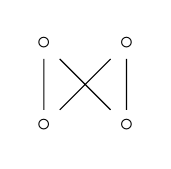
\begin{tikzpicture}[scale=.7]
        \node (a) at (0,1.5) {$\circ$};
        \node (b) at (0,0) {$\circ$};
        \node (c) at (1.5,1.5) {$\circ$};
        \node (d) at (1.5,0) {$\circ$};
        \draw (a) -- (b) -- (c) -- (d) -- (a);
      \end{tikzpicture}
      \caption*{${}_4C_2=6$}
    \end{subfigure}
  \end{figure}  
\end{example}
\subsection{Ideals and Filters イデアルとフィルター}
\begin{dfn}[Ideal]
  An \itbf{ideal} in a bounded distributive lattice $L$ is a subset $J \subseteq L$ such that
  \begin{eqnarray}
    \label{eq:ideal}
    && 0 \in J,\\
    && a,b \in J \Rightarrow a \vee b \in J,\\
    && b\le a \;\&\; a \in J \Rightarrow b \in J.
  \end{eqnarray}
\end{dfn}
\begin{dfn}[Filter]
  A \itbf{filter} in a bounded distributive lattice $L$ is a subset $F \subseteq L$ such that
  \begin{eqnarray}
    \label{eq:filter}
    && 1 \in F,\\
    && a,b \in F \Rightarrow a \wedge b \in F,\\
    && b \ge a \;\&\; a \in F \Rightarrow b \in F.
  \end{eqnarray}
\end{dfn}
\section{Stone Spaces}
\section{Spaces and Lattices of Open Sets}
We will suppose that all topological spaces that appear here will be $T_0$.
\subsection{Sober spaces}
\begin{dfn}[meet-irrducibility]
  Let $(X,\tau)$ be a top.space. $W\in \tau$ is said to be a \itbf{meet-irreducible} open set if $U,V\in \tau$ and $U \cap V \subseteq W$, then either $U \subseteq W$ or $V \subseteq W$.
\end{dfn}
\begin{dfn}[sober space]
  $X$ is said to be \itbf{sober} if all the meet-irreducible open sets are of the form $X\backslash \overline{\{x\}}$.
\end{dfn}
\begin{prop}
  Each Haudorff space is sober.
\end{prop}
\begin{proof}
  Suppose $W$ is meet-irreducible, for contradiction, there exists $x_1,x_2\notin W$ and $x_i \in U_i, x_j \notin U_i(i \ne j)$.
  Then $W = (W \cup U_1) \cap (W \cup U_2)$ and $W\cup U_i \nsubseteq W$.
\end{proof}

% ---REFERENCES---%
\begin{thebibliography}{10}
\bibitem[Gratzer]{Gratzer}
  George A. Gratzer, 2009, Lattice Theory: First concept and distributive lattices, Dover Publications.
\bibitem[Picado]{Picado}
  Jorge Picado, Ale\u{s} Putlr, Frames and Locales:Topology without points, Birkh\"auser.
\bibitem[Stone]{Stone}
  Peter T. Johnstone, Stone Spaces, Cambridge University Press.
\bibitem[Willard]{Willard}
  Steven Willard, General Topology, Dover Publications
\end{thebibliography}

\end{document}
